\chapter{Model}
\label{Model}


\section{Model}
\label{sec:Model}
Sketch two realistic scenarios for DarkSense to work in:\\
- The ewi hallway
- A street light

\subsection{Hallway}
explain environment (222 cm wide, 2,8m high, Lit as in ewi).\\
Show that the room can be lit in a similar way with the light im going to use in section \ref{sec:Method}.\\
Show what an signal would look like if a person walked trough the hallway underneath the light.\\
Show that the amount of light expected is 70Lx (place holder number), and that the proportional difference ranges from $\pm 0.5\%$ to $5\%$.
Calculated the speed of the person.\\
Approximate this signal as a function of Time and light emitted by the led\\
$ Person_{Hallway} = I_{NoObject} * [ProportionalDifference] * sin(t*2\pi f) + I_{NoObject}$\\
where s = proportional difference.\\

show approximation in figure with modelled signal\\

\subsection{StreetLight}
Explain environment (2m side walk, 6m street, lit as in "Handboek bestaande bouw" \cite{HandboekBestaandeBouw}.\\
Show what kind of light is required to do this\\
Show what an signal would look like if a person walked trough over the walkway\\
Show what a signal would look like if a car drove by in both of the drive lanes (1.5m and 4.5m distance of the light)\\
Show that the amount of light expected is 1Lx (place holder number), and that the proportional difference ranges from $\pm 0.5\%$ to $5\%$.\\
Calculate the speed of a person and a car\\
Approximate these signals.\\
$ Person_{street} = I_{NoObject} * s * sin(t*2\pi f) + I_{NoObject}$\\
$ Car_{street} = I_{NoObject} * s * sin(t*2\pi f) + I_{NoObject}$\\
where s = proportional difference.\\

show approximations in figure with modelled signal\\


\begin{figure}[!h]
	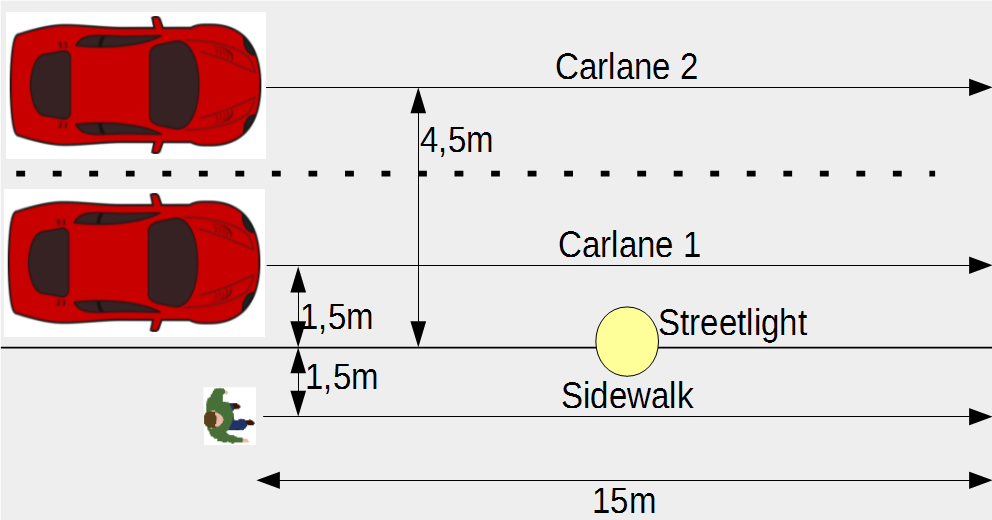
\includegraphics[width=\textwidth]{pics/streetlightoverview.png}
	\caption{Overview of the simulated street.}
	\label{fig:simulatedStreet}
\end{figure}

\begin{figure}[!h]
	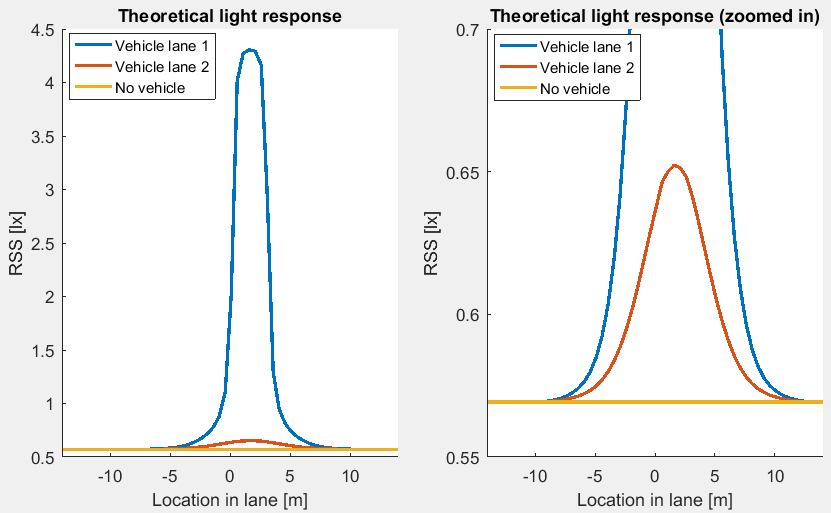
\includegraphics[width=\textwidth]{pics/CarDriveBy.png}
	\caption{Results of the drive-by simulation.}
	\label{fig:CarDriveBy}
\end{figure}


\section{Method}
\label{sec:Method}


\begin{figure}[!h]
	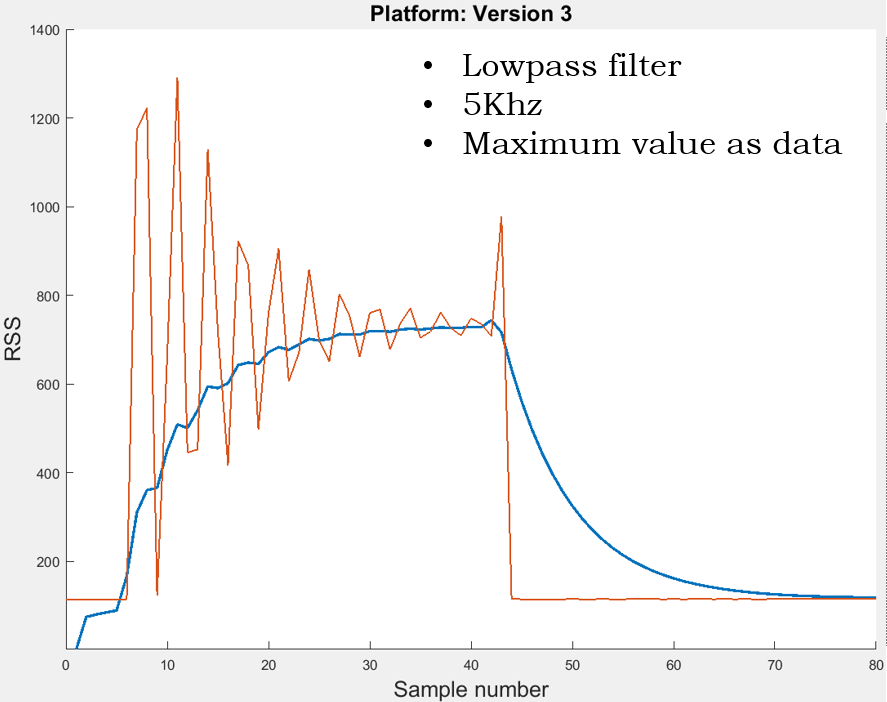
\includegraphics[width=\textwidth]{pics/66KhzFilter_placeholder.png}
	\caption{The data captured by the system before and after filtering. @=PLACEHOLDER FIGURE!@.}
	\label{fig:66KhzFilter}
\end{figure}

\subsection{Ideal T-on Time}
\label{subsec:T-on_Time}
Show several filtered captured signals in one figure\\
point out the part where light becomes constant\\
pick that t-on time as minimum\\
Mention that a sample of darkness can be taken @ 80 samples.\\
That the number (80) can be reduced by picking a FIR filter instead (less ripple)\\

\subsection{noise}
\label{subsec:noise}
Show the result of several "filtered flashes".\\
Explain sources of the "noise", also show FFT and histogram of the noise\\
Explain that the noise could be reduced, but that this would cost a lot more processor time. (which is not recommended to run at 125Hz).\\
Note the noise is approximately Gaussian.

\begin{figure}[!h]
	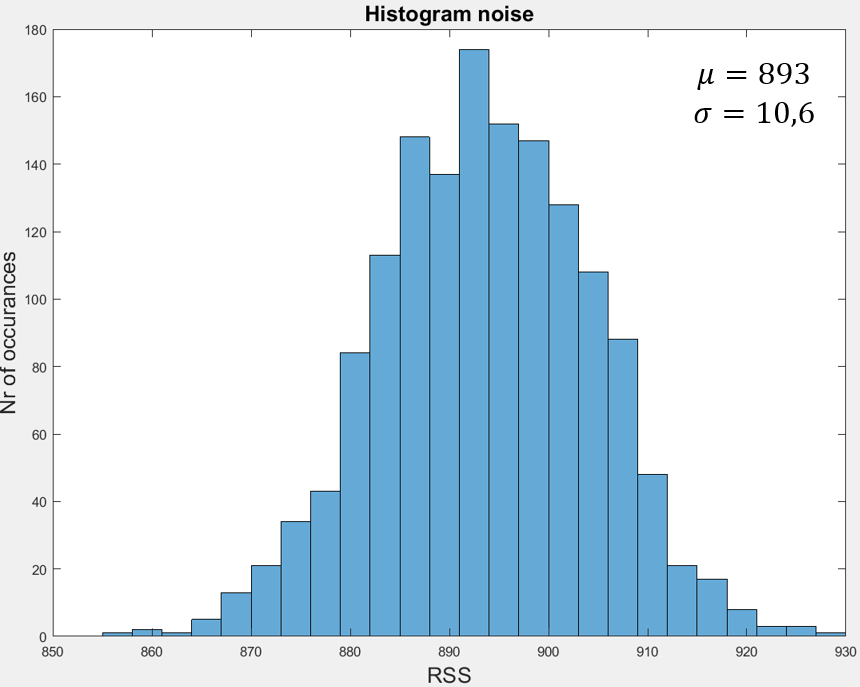
\includegraphics[width=\textwidth]{pics/histogram_noise_placeholder.png}
	\caption{Histogram of the noise of the data sampled by the system. The distribution roughly follows a normal curve. @=PLACEHOLDER FIGURE!@.}
	\label{fig:histogram_noise}
\end{figure}

